\subsection{Negation}
\label{subsec:fundamentals_negation}

Negationen sind wesentlich, weil wir mit ihnen das Gegenteil einer Aussage
präzise ausdrücken und dadurch logische Zusammenhänge systematisch untersuchen
können.

\begin{DefinitionBox}{Negation}{fundamentals_negation}
  Die \emph{Negation} \EnglishTerm{negation} einer Aussage $A$ wird mit
  $\neg A$ bezeichnet und kehrt den Wahrheitswert von $A$ um: Ist $A$ wahr, so
  ist $\neg A$ falsch; ist $A$ falsch, so ist $\neg A$ wahr.
\end{DefinitionBox}

\begin{ExampleBox}{Negation von Aussagen}{fundamentals_negation_example}
  Negieren Sie jeweils die angegebene Aussage $A$.
  \begin{enumerate}[label=(\alph*),itemsep=0.8em]
    \item Für eine feste reelle Zahl $x$:
      \par\smallskip
      \makebox[1.5cm][l]{$A:$}$x>5$\\[0.4em]
      \makebox[1.5cm][l]{$\neg A:$}\Cloze{5cm}{$x\leq 5$}

    \item
      \par\smallskip
      \makebox[1.5cm][l]{$A:$}„Die Zahl $17$ ist eine Primzahl.“\\[0.4em]
      \makebox[1.5cm][l]{$\neg A:$}\Cloze{9cm}{„Die Zahl $17$ ist keine Primzahl.“}

    \item
      \par\smallskip
      \makebox[1.5cm][l]{$A:$}„Heute regnet es.“\\[0.4em]
      \makebox[1.5cm][l]{$\neg A:$}\Cloze{9cm}{„Heute regnet es nicht.“}
  \end{enumerate}
\end{ExampleBox}

Wendet man eine Negation auf eine UND- oder ODER-Verknüpfung an, so muss man die
de-morganschen Regeln berücksichtigen. Mit dem zuvor eingeführten
Äquivalenzzeichen lassen sich diese präzise formulieren.

\begin{TheoremBox}{De-morgansche Regeln}{fundamentals_de_morgan_rules}
  Beim Negieren einer Verknüpfung werden UND und ODER miteinander vertauscht
  und beide Teilaussagen negiert:
  \[
    \neg(A\land B)\Leftrightarrow (\neg A)\lor(\neg B),
  \]
  \[
    \neg(A\lor B)\Leftrightarrow (\neg A)\land(\neg B).
  \]
\end{TheoremBox}

\begin{ExampleBox}{De-morgansche Regeln}{fundamentals_de_morgan_rules_example}
  Es seien $a,b,x\in\R$ mit $a\leq b$. Nach der zweiten de-morganschen Regel
  gilt
  \begin{align*}
    \neg\bigl((x<a)\lor(x>b)\bigr)
      &\Leftrightarrow
        \Cloze{7.2cm}{\neg(x<a)\land\neg(x>b)}\\
      &\Leftrightarrow
        \Cloze{7.2cm}{(x\geq a)\land(x\leq b)}.
  \end{align*}

  \begin{center}
    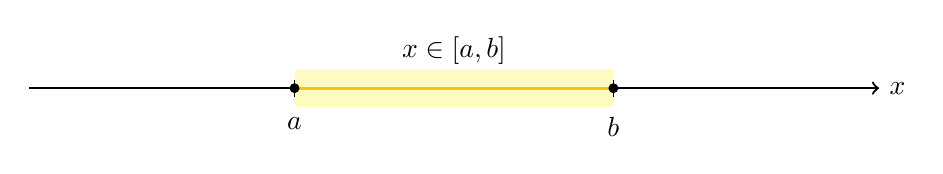
\begin{tikzpicture}[x=1.35cm,y=1cm]
  \fill[yellow!70,opacity=0.35] (-1.5,-0.24) rectangle (1.5,0.24);
  \draw[->,thick] (-4,0) -- (4,0) node[right] {$x$};
  \draw[very thick,yellow!55!orange] (-1.5,0) -- (1.5,0);
  \fill (-1.5,0) circle (1.8pt);
  \fill (1.5,0) circle (1.8pt);
  \draw (-1.5,0.11) -- (-1.5,-0.11) node[below=4pt] {$a$};
  \draw (1.5,0.11) -- (1.5,-0.11) node[below=4pt] {$b$};
  \node[above=5pt] at (0,0) {$x\in[a,b]$};
\end{tikzpicture}

  \end{center}

  Die ursprüngliche Aussage schließt aus, dass $x$ links von $a$ oder rechts
  von $b$ liegt. Daher muss gleichzeitig $x\geq a$ und $x\leq b$ gelten. Dies
  ist genau der auf dem Zahlenstrahl markierte Bereich $x\in[a,b]$; die
  Randpunkte gehören dazu, weil die strengen Ungleichungen $x<a$ und $x>b$
  negiert werden.
\end{ExampleBox}
